\section{Lezione 10}%
\label{sub:Lezione 10}
\subsection{Random Walk di Weierstrass nel dettaglio}%
\label{sub:Random Walk di Weierstrass nel dettaglio}
Abbiamo visto che per un camminatore di Weierstrass la forma della distribuzione poteva non essere Gaussiana al variare del parametro $N^2 / b$ (Vedi sezione \ref{sub:Random Walk di Weierstrass}). \\
Cerchiamo la distribuzione invariante per il camminatore di Weierstrass. La probabilità di fare un salto $l$ abbiamo visto essere:
\[\begin{aligned}
    P(l) = \frac{M-1}{2M}\sum_{J=0}^{\infty} \frac{1}{M^J}\left[\delta (l-b^Ja) + \delta (l+b^Ja) \right]
.\end{aligned}\]
In generale la probabilità di fare un salto $ba$ è soppressa di un fattore $1 /M$ rispetto a quella di saltare $a$, questo comporta che:
\begin{itemize}
    \item Occorrono $\sim M$ salti di $\pm a$ prima di saltare $ba$.
    \item Occorrono $\sim M$ salti di $\pm ba$ ($M^2$ salti lunghi $a$) prima di saltare $b^2a$.
    \item etc \ldots
\end{itemize}
Queste caratteristiche fanno si che il sistema esibisca dei cluster di camminatori attorno alle posizioni dei salti lunghi.
\begin{figure}[H]
    \centering
    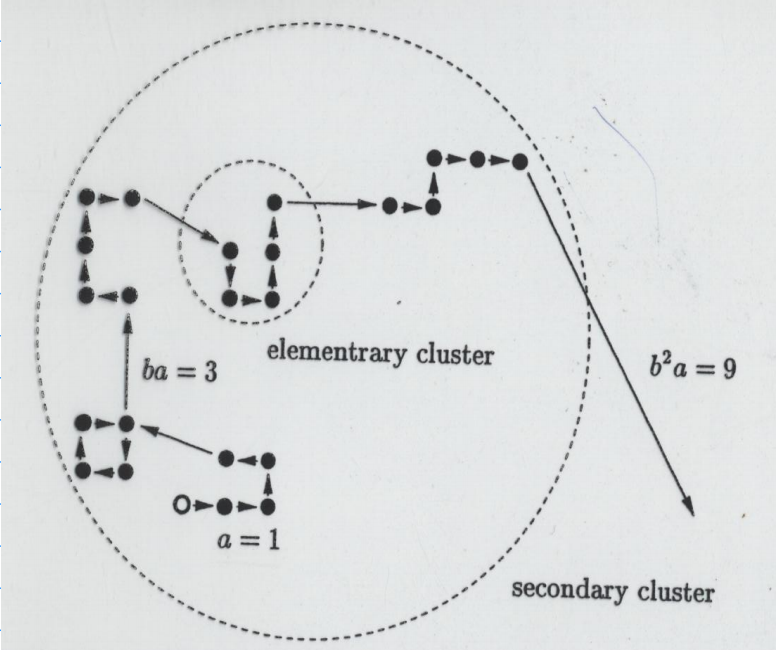
\includegraphics[width=0.4\textwidth]{figures/10_RWWeierstrass.png}
    \caption{\scriptsize Random Walk di Weierstrass ($b=3$, $M=4$): formazione dei Cluster (Paul and Baschangel: Stochastic Process, Springer).}
    \label{fig:figures-10_RWWeierstrass-png}
\end{figure}
\noindent
Proprio per la formazione di questi cluster su scale spaziali diverse il sistema può presentare un comportamento auto-similare.\\
Possiamo notare anche come cambiano i risultati al variare dei parametri $M$ e $b$:
\begin{figure}[H]
    \centering
    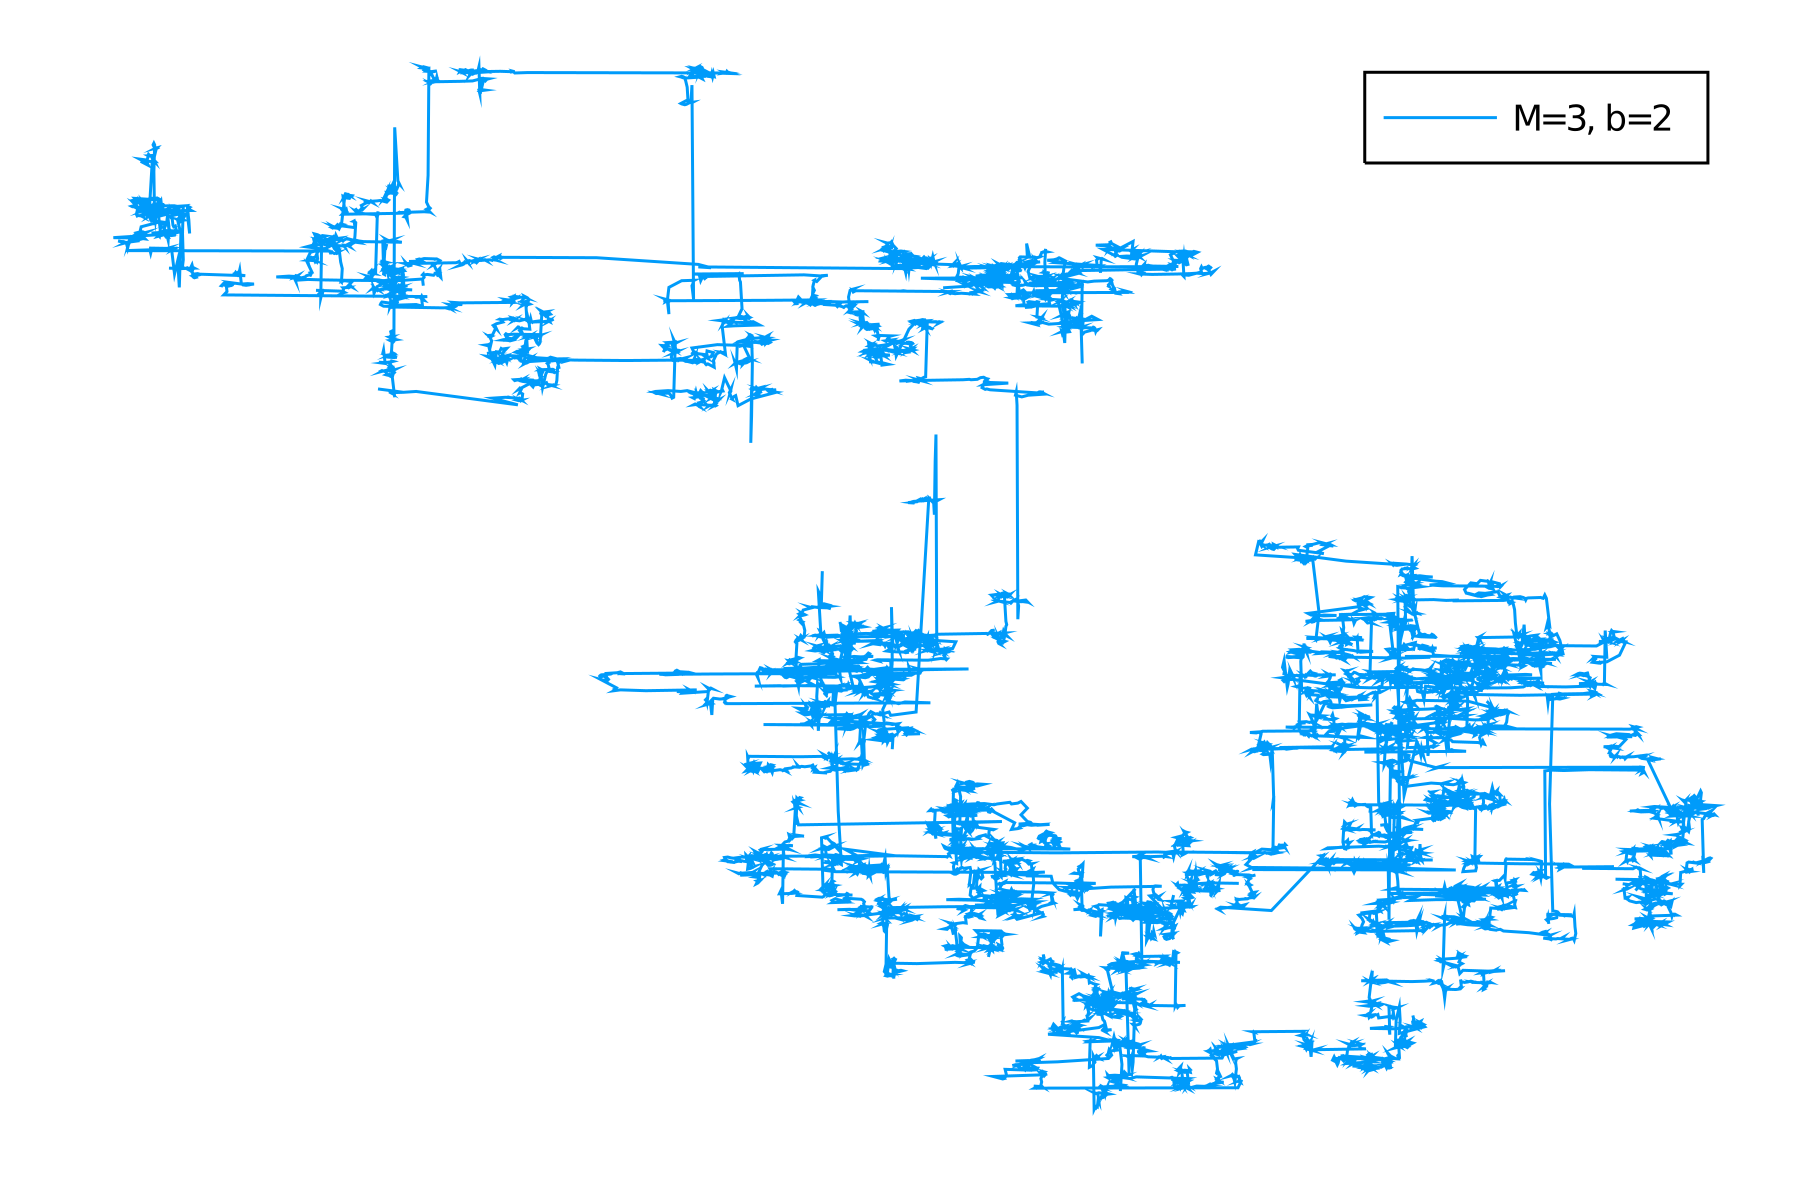
\includegraphics[width=0.45\textwidth]{figures/lez_10_Weier_M_3_b_2.png}
    \caption{\scriptsize Rapporto $M^2 / b = 4.5$.}
    \label{fig:figures-lez_10_Weier_M_3_b_2-png}
\end{figure}
\begin{figure}[H]
    \centering
    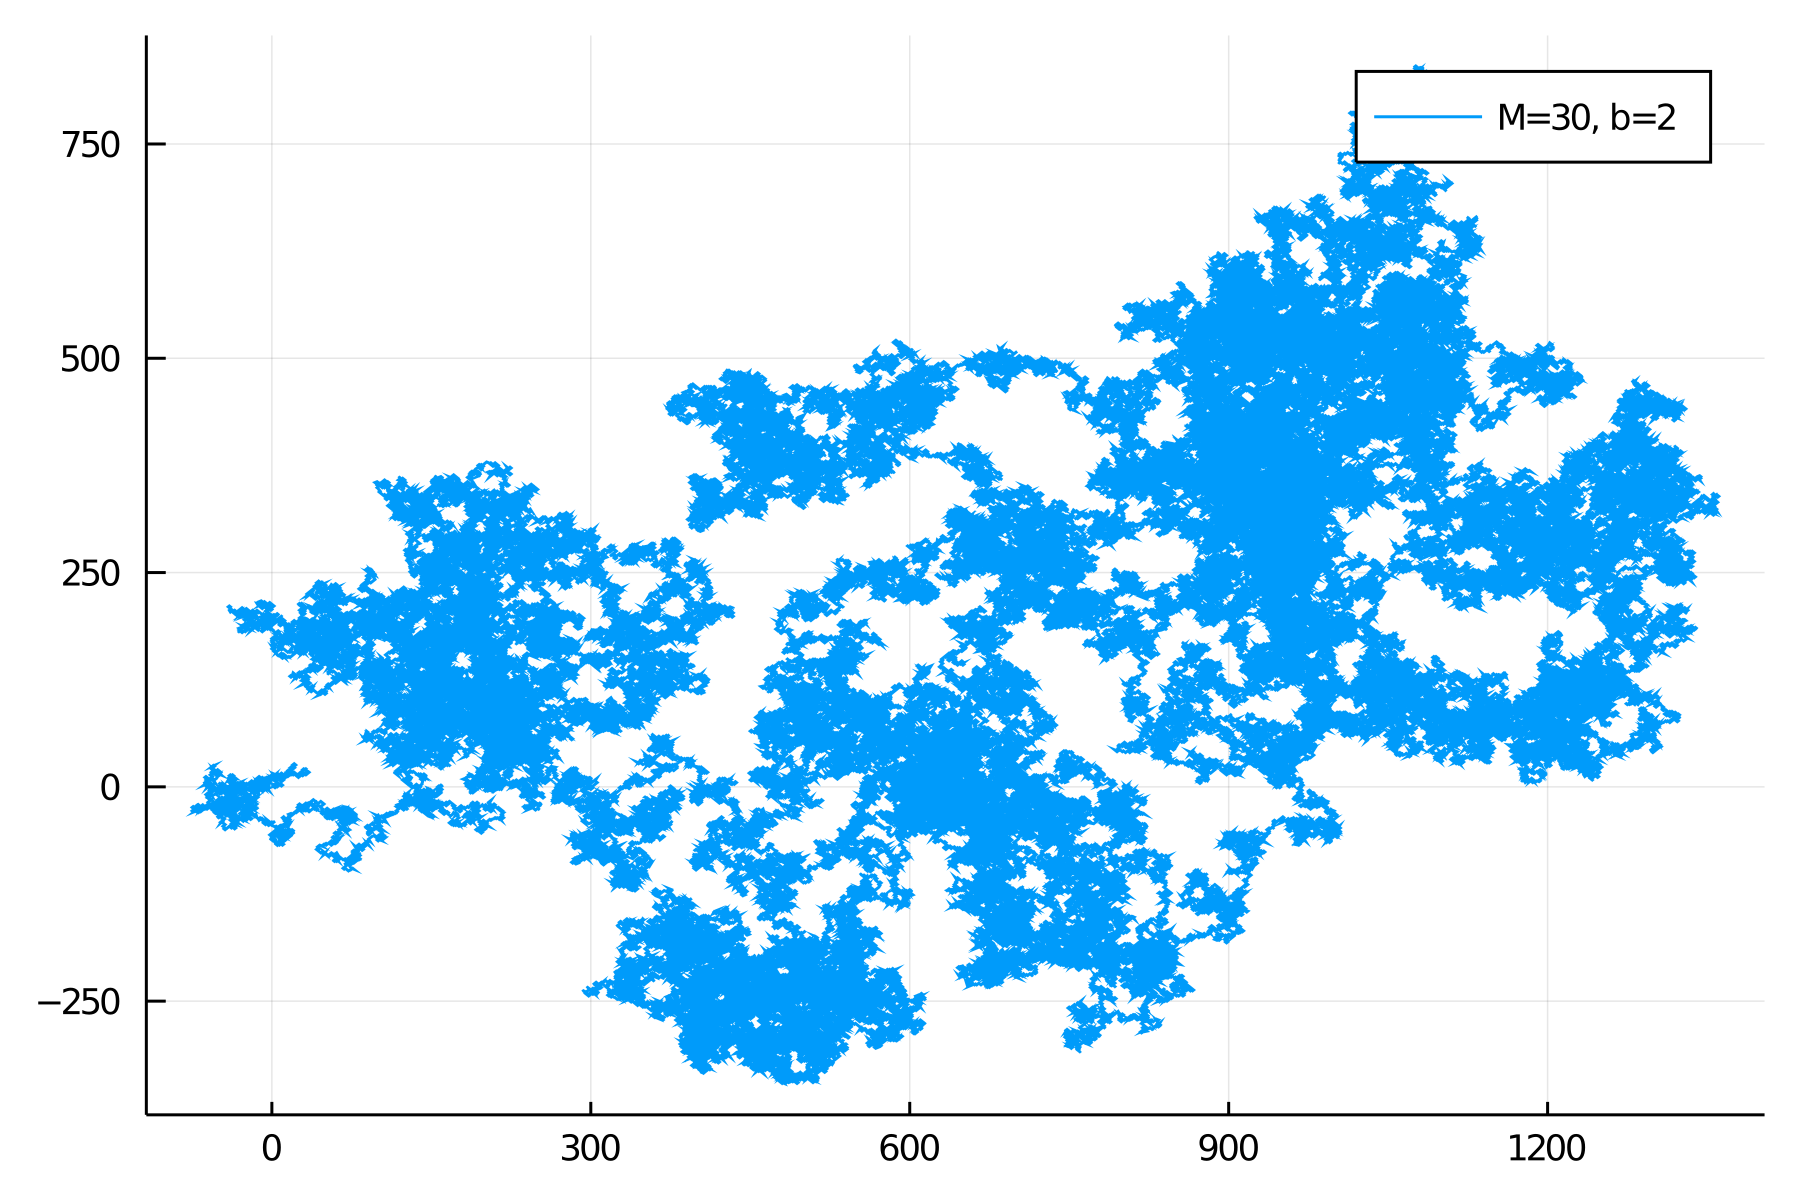
\includegraphics[width=0.45\textwidth]{figures/lez_10_Weier_M_30_b_2.png}
    \caption{\scriptsize Rapporto $M^2 / b = 450$, notiamo come i cluster che si formano siano diversi nei due casi.}
    \label{fig:figures-lez_10_Weier_M_3_b_2-png}
\end{figure}

Risolviamo per $\left<l^2\right>\to 0$, quindi il caso in cui la distribuzione $P(l)$  non può tendere ad una Gaussiana.
\[
    \left<l^2\right> = \frac{\left(M-1\right)a^2}{M}\sum_{}^{} \left(\frac{b^2}{M}\right)^J; \quad \frac{b^2}{M}>1
.\] 

